\documentclass[12pt,a4paper]{report}
\usepackage[utf8]{inputenc}
\usepackage[T1]{fontenc}
\usepackage{amsmath}
\usepackage{amsfonts}
\usepackage[english,russian]{babel}
\usepackage{amssymb}
\usepackage{graphicx}
\graphicspath{{pictures/}}
\DeclareGraphicsExtensions{.pdf,.png,.jpg}

\usepackage{hyperref}

\begin{document}
	\begin{center}
		{\large\bf УЧЕБНАЯ ПРАКТИКА.\\
			ПРАКТИКА ПО ПОЛУЧЕНИЮ ПЕРВИЧНЫХ  ПРОФЕССИОНАЛЬНЫХ УМЕНИЙ И НАВЫКОВ, В ТОМ ЧИСЛЕ ПЕРВИЧНЫХ УМЕНИЙ И НАВЫКОВ НАУЧНО-ИССЛЕДОВАТЕЛЬСКОЙ ДЕЯТЕЛЬНОСТИ}\\
		{\it Новиков Е.А.}
	\end{center}
	
	\newpage
	
	\section{Работа, проделанная в период 30.10.2020 - 5.11.2020}
	3.11.2020 Осуществил разбор первой главы книги Наоми Седер "Python. Экспресс-курс". Шло повествовании о плюсах и минус языка Python. Рассказывалось, для чего он полезен и как вынести из него максимальную выгоду. Перешёл ко второй главе. В ней стали описывать "лёгкую" разработку программ в python. Установил PyCharm. Добавил переменные среды. Столкнулся с проблемой некомпилируемой обработки программы ">>> print("Hello, World")". Ошибка 9009. Попытался разобраться сам. Проблема не решилась после переустановки и новой переменной среды. Начал поиск в интернете. Нечего нового не нашёл.

	4.11.2020 Вновь попытался найти полезную информацию в Интернете. Ещё раз переустановил PyCharm. ToolBox перестал его запускать, а только предлагает его переустановить. PyCharm запускается единственным способом - через панель меню "Пуск". Закончил разбор второй главы книги Наоми Седер "Python. Экспресс-курс".
	
	\section{Работа, проделанная в период 06.11.2020 - 12.11.2020}
	9.11.2020 Освоил главу 3. Понял, что знак ">>>" относится к консоли python, а не к коду. Начал главу 4.

	10.11.2020 Дочитал главу 4, сделал задания для лучшего освоения. \url{https://yadi.sk/d/7tAiVBXUr4HP0g?w=1}. Просмотрел лекции Введение, "Искусственные нейронные сети", "Обучение нейронных сетей".

	11.11.2020 Освоил главу 5. Не смог найти файл с лабораторной работы в конце этой главы. \url{https://yadi.sk/d/YZpACJ_52mXBFA?w=1(5.3?)}. Лекции "Библиотеки для глубокого обучения", "Распознавание предметов одежды", "Анализ качества обучения нейронной сети".
	
	\section{Работа, проделанная в период 13.11.2020 - 20.11.2020}
	Определение 

Нейросеть  - это модель обработки информации, которая призвана автоматизировать, упрощать и ускорять работу человека. Она действует так же, как и биологические нервные системы человека, созданные для обработки информации. 

 Типы нс: 

\begin{enumerate}
\item Сверточные сети - одни из самых популярных типов искусственных нейронных сетей. Они доказали свою эффективность в распознавании визуальных образов (видео и изображения), рекомендательных системах и обработке языка.

Сверточные нейронные сети отлично масштабируются и могут использоваться для распознавания образов, какого угодно большого разрешения.
В этих сетях используются объемные трехмерные нейроны. Внутри одного слоя нейроны связаны лишь небольшим полем, названые рецептивным слоем.
Нейроны соседних слоев связаны посредством механизма пространственной локализации. Работу множества таких слоев обеспечивают особые нелинейные фильтры, реагирующие на все большее число пикселей.

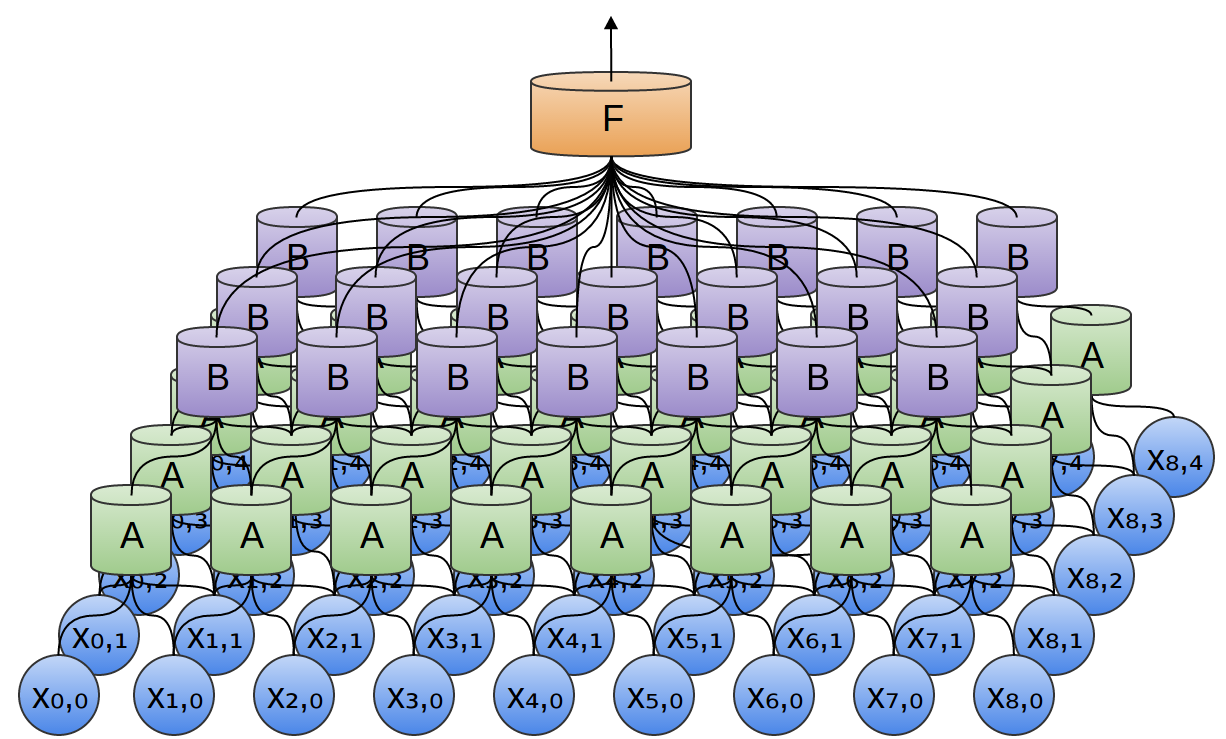
\includegraphics{sv}

\item Сеть с прямым распространением сигналов. В ней запрещены циклы. Сначала сигнал передаётся на скрытый слой, затем на выходной слой и во внешнюю среду. Xасто описываtтся в виде слоёного торта, где каждый слой состоит из входных, скрытых или выходных клеток. Клетки одного слоя не связаны между собой, а соседние слои обычно полностью связаны. Если у сети есть достаточное количество скрытых нейронов, она теоретически способна смоделировать взаимодействие между входным и выходными данными. Практически такие сети используются редко, но их часто комбинируют с другими типами для получения новых.

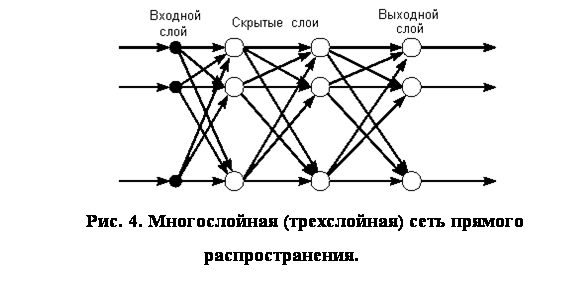
\includegraphics{pr}
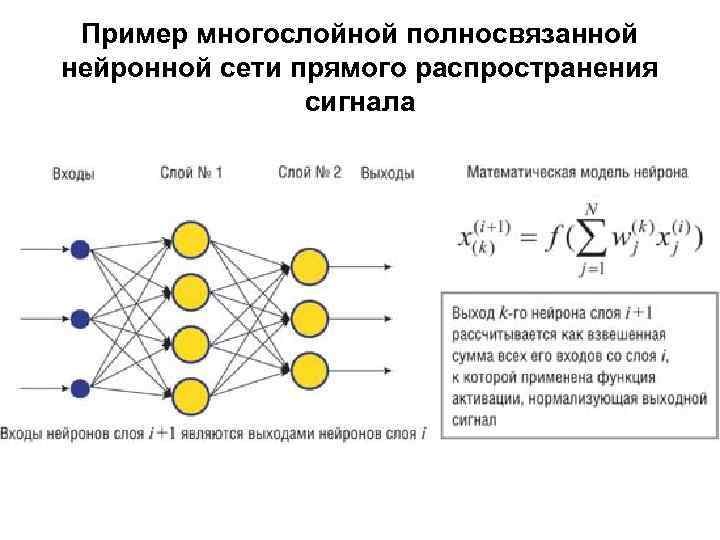
\includegraphics{pr2}

\item Рекуррентная сеть – сеть в которой возможны циклы. Здесь сигнал от входного может поступать на любой из скрытых слоёв из скрытого слоя или даже на предыдущий слой. Её можно представить в виде сети с прямым распространением сигнала во времени. В данной нс у каждого соединения есть свой вес, он же приоритет. Узлы в ней делятся на два типа, вводные узлы и узлы скрытые. Информация в рекуррентной нейронной сети передается не только по прямой, слой за слоем, но и между самими нейронами. Важной отличительной особенностью рекуррентной нейронной сети является наличие так званой «области внимания», когда машине можно задать определенные фрагменты данных, требующие усиленной обработки.

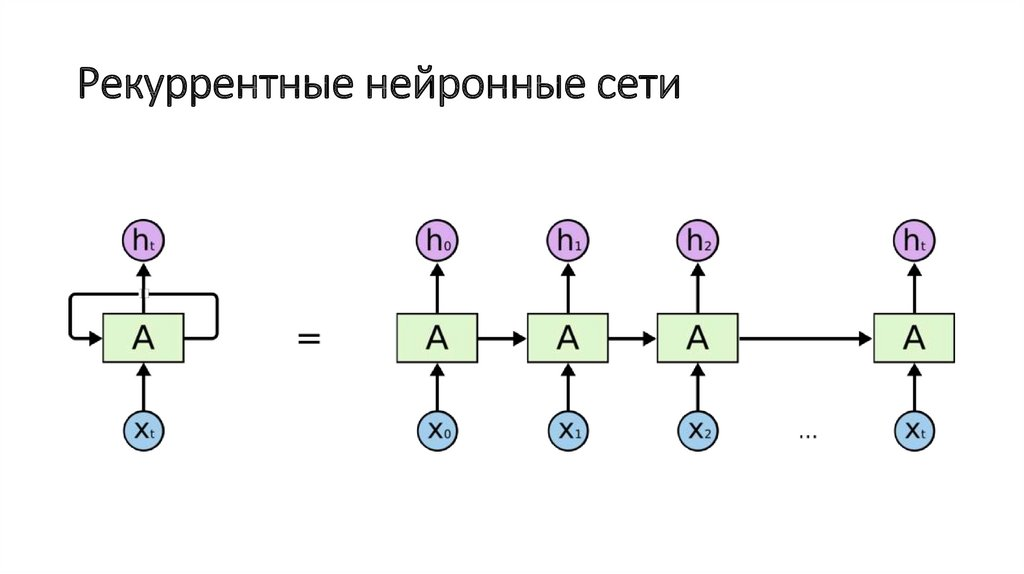
\includegraphics{rek}
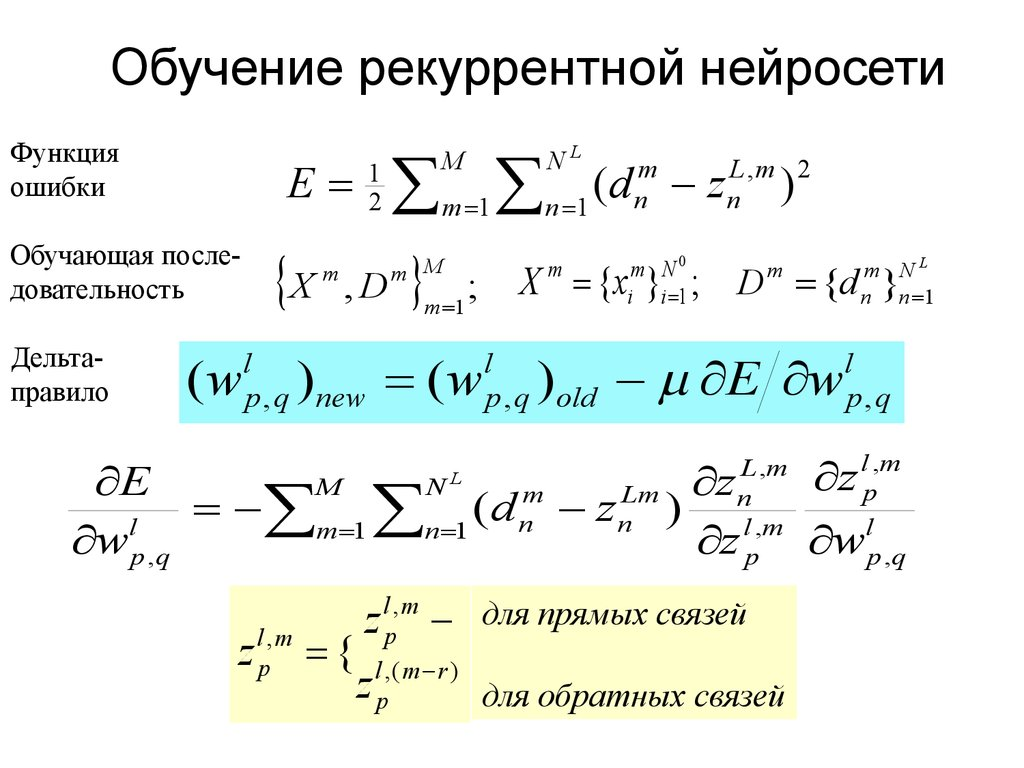
\includegraphics{rek2}

\end{enumerate}

Сети, у которых больше одного скрытого слоя называются глубокими нейронными сетями. 

Методы обучения:
\begin{enumerate}
	\item Обучение с учителем. Должен быть набор данных, которые подаются на вход нейронных сетей для которых заранее известен правильный ответ;
	\item Обучение без учителя. Есть данные, но правильный ответ для них заранее не известен;
	\item Обучение с подкреплением. Получает сигналы и ответы от внешней среды.
\end{enumerate}


 Методы поиска оптимальных весов 

Полное обучение. анализ ошибки на всех элементах данных, подсчёт направления градиента и только потом изменяем веса. Но если данных много, этот метод не будет эффективен.  

Онлайн обучение, это когда мы делаем шаг в сторону изменения, когда обработали один элемент данных или нескольких элементов данных (мини-выборки). В таких случаяхх на разных этапах обучения мы можем двигаться в разные стороны, в том числе, ошибка может увеличиваться. Но если данных много, а размер шага в сторону градиента маленький, то со временем мы дойдём до минимального значения функции ошибки. 

 Метод обратного распространения ошибки 

При обучении с учителем, нам нужно знать ошибку не только на выходном слое, но и на выходе всех скрытых слоёв и на входном слое. Зная ошибку на выходном слое, мы рассчитываем ошибку поочерёдно на скрытых слоях, затем на входном слое. Если мы знаем ошибку на выходе, мы можем получить ошибку на входе. Пусть у нас есть скрытый слой и мы получили ошибку на выходе. Если нейрон линейный, нам нужно взять значение на выходе из нейрона и умножить на вес этого выхода.  

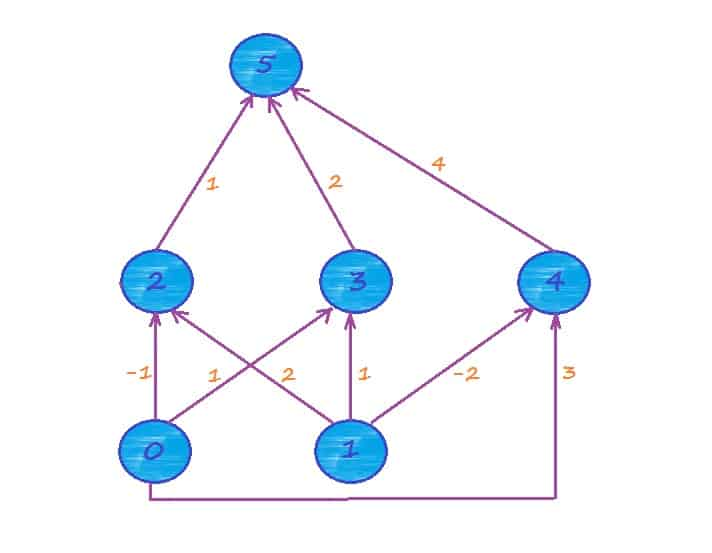
\includegraphics{weight}
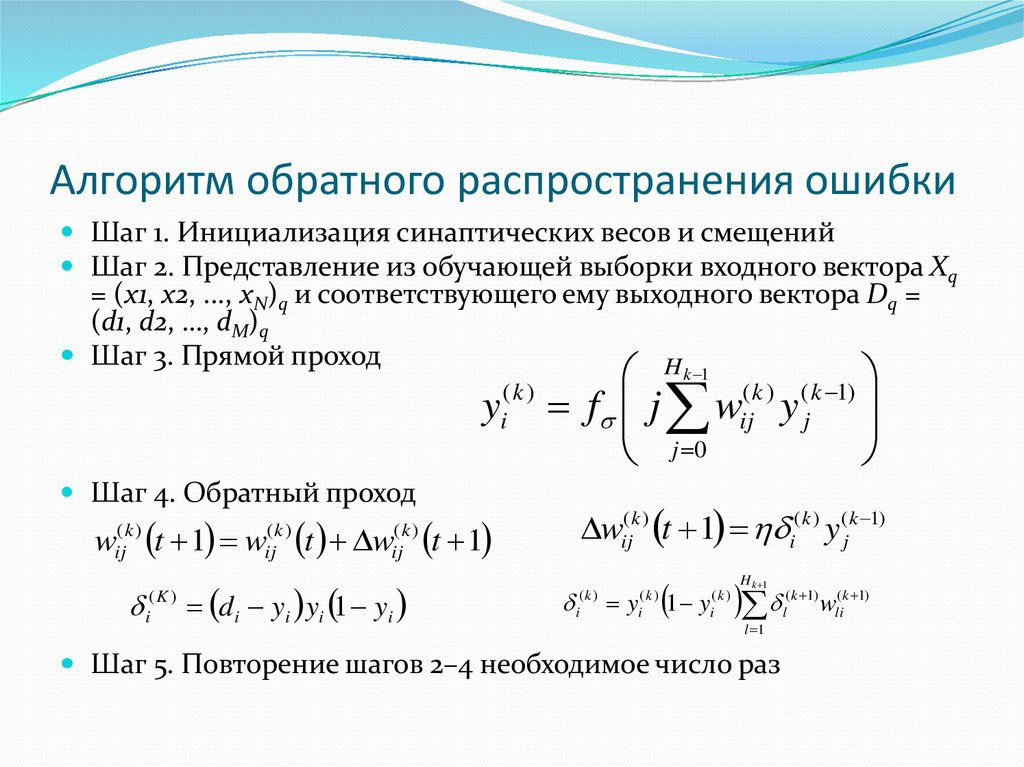
\includegraphics{weight2}



\end{document}
